\label{ch:fem}
As a conclusion of the previous chapter one can see that the number of methods that are currently available to describe a FEF in presence of an intricate electrostatic background potential is not that large.
In this work, the method of choise to model the free electron function is the FEM which has been applied to quantum-mechanical problems by several authors \cite{fem_hydro, vib_fem, fe_hf, fe_dft1}.
However, to the best of my knowledge, only the bound state problems were addressed so far.
A brief review of these works is given in section \ref{ch:feQM}.
Besides its large flexibility and computational efficiency pointed out in section \ref{ch:introFEM}, the large amount of available FEM libraries \cite{libmesh,dealII,freefem, hermes,oofem} that are developed mainly for engineering problems is another advantage of practical importance due to the complexity of the generation of a suitable mesh, assembling of matrices and solution of matrix equations.

In the following chapter, the integration of the matrix elements (section \ref{ch:feInt}) and set up of the mesh (section \ref{ch:feAss}) will be described.
Thereby the focus is put on the application to the one-particle SE that is to be solved with molecular electrostatic potential (ESP).
Since the interest thereby is on free particle solutions, the spectrum is expected to be very dense and the wave function to be delocalised, requiring well-designed boundary conditions.
A discussion of various boundary conditions and mimicing asymptotic behaviour available for FEM is described in section \ref{ch:BC}.

%\section{Finite Element Calculations in Quantum Chemistry}
\section{Finite Element Methods for Electronic Structure Calculations}
\label{ch:feQM}
The FEM is mainly known from engineering disciplines where it is used in a broad range of applications such as modelling of fluids \cite{fluid1,fluid2}, heat transfer and flow \cite{heat1, heat2,heat3} or material deformation under mechanical stress \cite{deform1, deform2}.
However, also several different quantum-mechanical problems have been addressed with this method: electronic structure methods for small systems such as light atoms \cite{fem_hydro,fem_He,fem_He1, fem_h1, LiGS_fem} or diatomics \cite{fem_H_refine}, model oscillator systems \cite{vib_fem} and solid state problems \cite{fem_crystal, fem_crystal1}.
Moreover, even Hartree-Fock \cite{fe_hf} and DFT calculations on systems up to the size of benzene \cite{fe_dft1, fe_dft2, fe_dft3} have been performed, yielding results comparable to those obtained by the usual LCAO approach.

The above-mentioned applications have shown that the FEM is able to obtain reasonable results for molecular systems where the errors were comparable to those obtained with standard quantum-chemistry schemes even though their computational costs are higher.
Here, usual quantum-chemical methods are more suited, since local basis functions localised on atoms are more convenient for bound problems.
This suggests however that the FEM should be a robust tool for the description of unbound states which represents a very non-trivial task for conventional techniques.

%\section{From Weak Form to a Matrix Equation}
%\section{Integration of Matrix Elements and Formulations of the Equation System}
\section{Setup of the Equation System}
\label{ch:feInt}
In section \ref{ch:introFEM} the basics of the FEM were described and the generalised eigensystem shown in \eq{eq:SEmat} for the SE was derived.
Here this is taken as starting point and a closer look at the computation of the matrix elements as well as solving strategies for the large sparse generalised eigenproblems are taken.

The generalised eigenproblem as given in \eq{eq:SEmat} consists of three matrices.
Since the ansatz functions (shape functions) $\varphi_i(\vec{r})$ have only a small support, most of the matrix elements are zero. 
However, in two and three dimensions no distinct band structure is achievable and the matrices are irreducible.
Thereby matrix elements are zero when the elements involved are not neighboured as can be followed from Figure \ref{fig:2Del} where a linear basis function of a 2D-mesh is shown.
The computation of the non-zero matrix elements involve an integration as, \textit{e.g.}, the overlap integral $\mat{M}_{i,j}=\int d \vec{r} \varphi_i(\vec{r}) \varphi_j(\vec{r})$ of ansatz functions.
In practice these integrals are performed on a standard reference element and than scaled according to the Jacobian of the respective linear transformation that transforms the reference element to the physical one.
Since these functions are the same for all elements, the evaluation of the integrals on the reference elements can be done via a lookup-table or an efficient numerical integration scheme whose order is given by the shape functions.
The matrix elements $\mat{A}_{i,j}=\int d \vec{r} \left(\nabla \varphi_i(\vec{r})\right)\left(\nabla \varphi_j(\vec{r})\right)$ consist of overlap integrals of known functions similar to those of $\mat{M}$.
The only matrix containing system-specific information is the potential $\mat{V}_{i,j}=\int d \vec{r} \varphi_i(\vec{r}) V(\vec{r}) \varphi_j(\vec{r})$ which requires numerical integration involving a reasonable approximation to $V(\vec{r})$ which can be obtained via interpolation of known points or using exact values computed at the given quadrature points.

After assembling the matrices the eigenpair $(e_i, \vec{c}_i)$ of the system
\begin{equation} \label{eq:SEmat2}
\left(\frac 12 \mat{A}+\mat{V}\right)\vec{c}_i = e_i \mat{M}\vec{c}_i
\end{equation}
need to be found, where the energy $e_i$ is the closest to the target kinetic energy of the photoelectron.
Since matrices with dimensions of several thousands typically occur, numerous schemes have been developed to solve them efficiently \cite{davidson,arnoldi, gpusolver,krylov}, and are described in section \ref{ch:ghep}.
Despite the numerical complexity because of the high dimensionality of this problem (several thousands of basis functions) the second problem is due to the fact that the eigenenergies $e_i$ are expected to be close to each other since the corresponding exact Hamiltonian has a continuous spectrum in this energy range.
It is well known in numerics that this leads to instabilities especially for the eigenvectors, making a regularisation of the problem (described in section \ref{ch:regular}) indispensable.

\section{Element Types and Mesh Types}
\label{ch:feAss}
Among the FEM formulations several flavours were designed for different purposes.
Given a certain equation to be solved in FEM, there are in general two systematic ways to increase the accuracy.
The first way is to increase the number of elements witch is referred to as the $h$-FEM approach \cite{dreyer,}.
The refinement of the mesh is in principle always possible but technically demanding since it is not known in which regions of a mesh are too coarse in general \cite{dreyer}.
To overcome this, some FEM implementations such as that of \prog{Libmesh} \cite{libmesh} which is used here, provide an iterative mesh refinement scheme, adapting the mesh using local error estimations and thus is fully automatic \cite{libmesh}.
However, theses schemes are numerically demanding and hence can be only applied to benchmark systems.

The second strategy is called $p$-FEM. 
In the $p$-FEM scheme, the order $p$ of the test functions in increased, resulting in smoother and more flexible solutions at the price of incrementing dimensionality \cite{p-fem}.
Standard FEM-libraries usually have only $p=1,2$ implemented, but high-order polynomials are also reported \cite{hermes}.
Combined schemes where the grid-size as well as the element order are adapted is referred to as $hp$-FEM \cite{hp-fem}.
These schemes are in principle promising but require detailed knowledge about the solution to setup the parameters reasonable in order to keep the computational demands in a feasible range.

Besides different refinement strategies, finite element types also vary in the way in which global smoothness is ensured and the numerical integration is obtained.
While for Lagrange elements the shape functions are evaluated at certain inner or boarder points, \textit{e.g.} in Argyris or Hsieh-Clough-Tocher elements also first or even second derivatives are evaluated \cite{femPraxis,femCiarlet}.
Moreover, one distinguishes conforming and the more general non-conforming meshes \cite{nonconfFEM}. In case of the latter, more general structures are supported as \textit{e.g.} hanging nodes which occur when a vertex of one element is on the edge of an other as illustrated in Figure \ref{fig:HexBenz} \cite{femCiarlet}.
The setup of the mesh is, as mentioned above already, critical to the quality of the solution and hence of special importance.
Moreover, it is technically non trivial to set up a close packing of volume elements with the desired properties in a systematic way.
Although in principle any element shape can be chosen, in three dimensions only tetrahedral (simplex), prism- and pyramid-shaped as well as hexahedral elements commonly are used.
By choosing the element shape and the polynomial order, the element type of shape functions are fully defined.
%When using hexahedral elements the ansatz functions usually are of the type $\varphi(\vec{r})=x^ky^lz^m$ where $p=k+l+m$ is the element order.

When considering meshes to describe molecular properties it is clear that the element size should be smaller in the vicinity of the nuclei while it may be larger at longer distances.
One way to create a hexahedral mesh with local refinement is to start with a coarse uniform lattice and subdivide the hexahedra where necessary as shown in Figure \ref{fig:HexBenz} for a benzene molecule.
Another way is to setup small regular cubic grids around the nuclei and expand them radially in boxes of growing size as shown in Figure \ref{fig:HexDia}.
These brick-shaped elements however have the disadvantages that the regular cube-like structures therein might be not well-suited for atoms and molecules having higher symmetries.
%Further hexahedral elements are known to give less accurate solutions than tetrahedra which are commonly used nowadays \textcolor{green}{cite}.
%\begin{wrapfigure}{r}{\textwidth}
%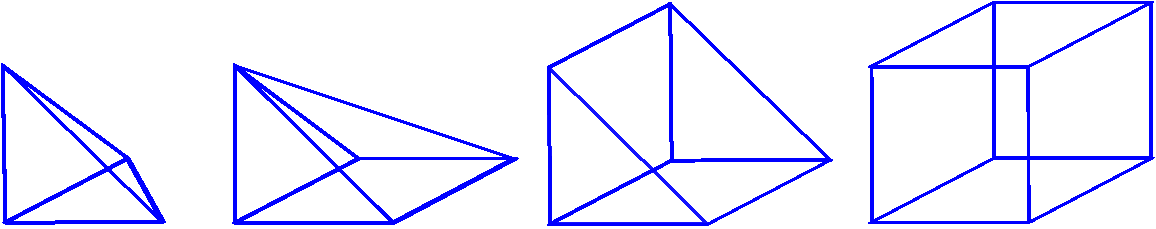
\includegraphics[width=\textwidth]{Figures/Elements3d-crop.pdf}
%\caption{The different Shapes of 3D elements.}
%\end{wrapfigure}

Another approach used by Lehtovaara \textit{et al.} \cite{fe_dft2} is to put layers of polyhedra around the atoms with increasing number of vertices and size.
Thereby the overlapping regions of these polyhedra are removed by excluding the vertices that are closer to a different atom.
\begin{figure}
  \begin{subfigure}{0.23\textwidth}
   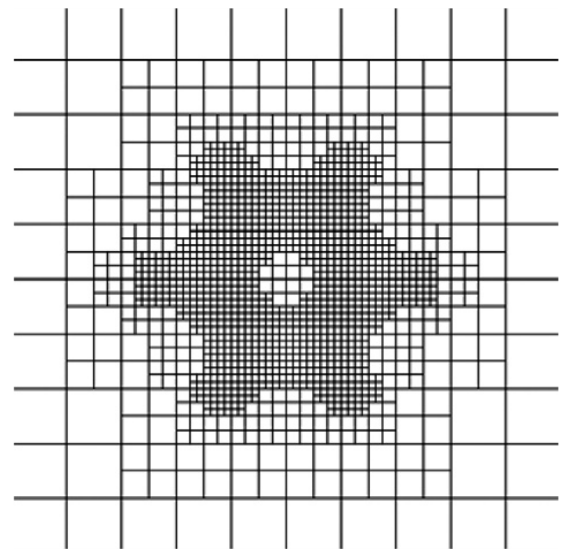
\includegraphics[width=\textwidth]{Figures/QuadMeshBenzene}
   \vspace{-43mm}\caption{$\qquad\qquad\qquad\qquad$}
   \label{fig:HexBenz}
  \end{subfigure}
  \begin{subfigure}{0.28\textwidth}
   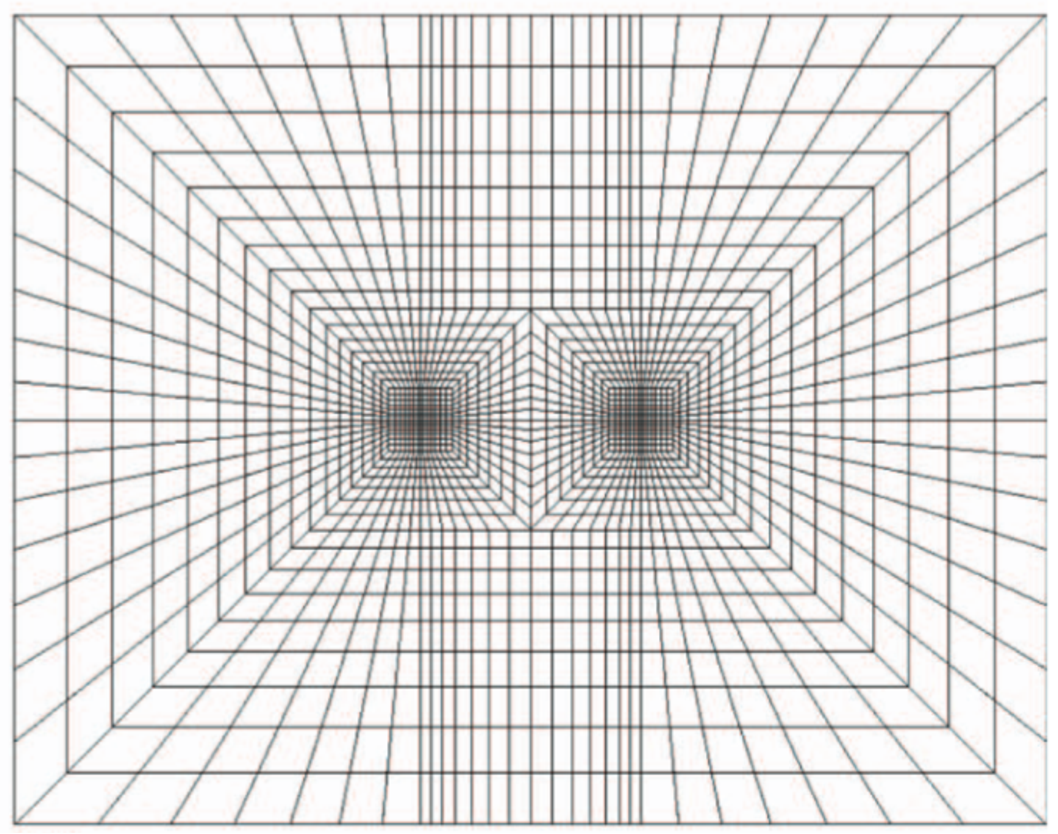
\includegraphics[width=\textwidth]{Figures/QuadDiatomic}
   \vspace{-43mm}\caption{$\qquad\qquad\qquad\qquad\quad$}
   \label{fig:HexDia}
  \end{subfigure}
  \begin{subfigure}{0.23\textwidth}
   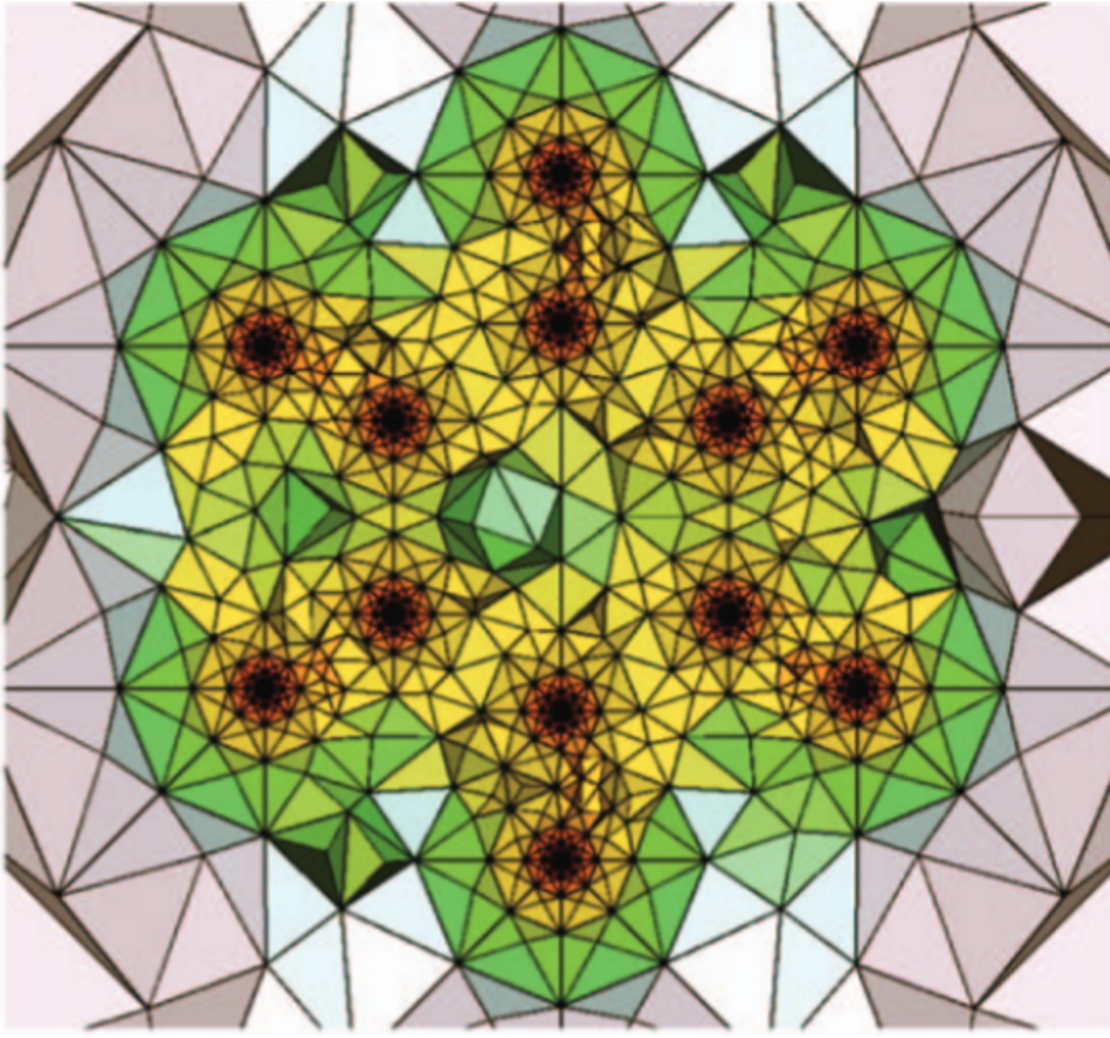
\includegraphics[width=\textwidth]{Figures/PolyBenzene}
   \vspace{-42mm}\caption{$\quad\qquad\qquad\qquad\quad$}
   \label{fig:PolyBenz}
  \end{subfigure}
  \begin{subfigure}{0.23\textwidth}
   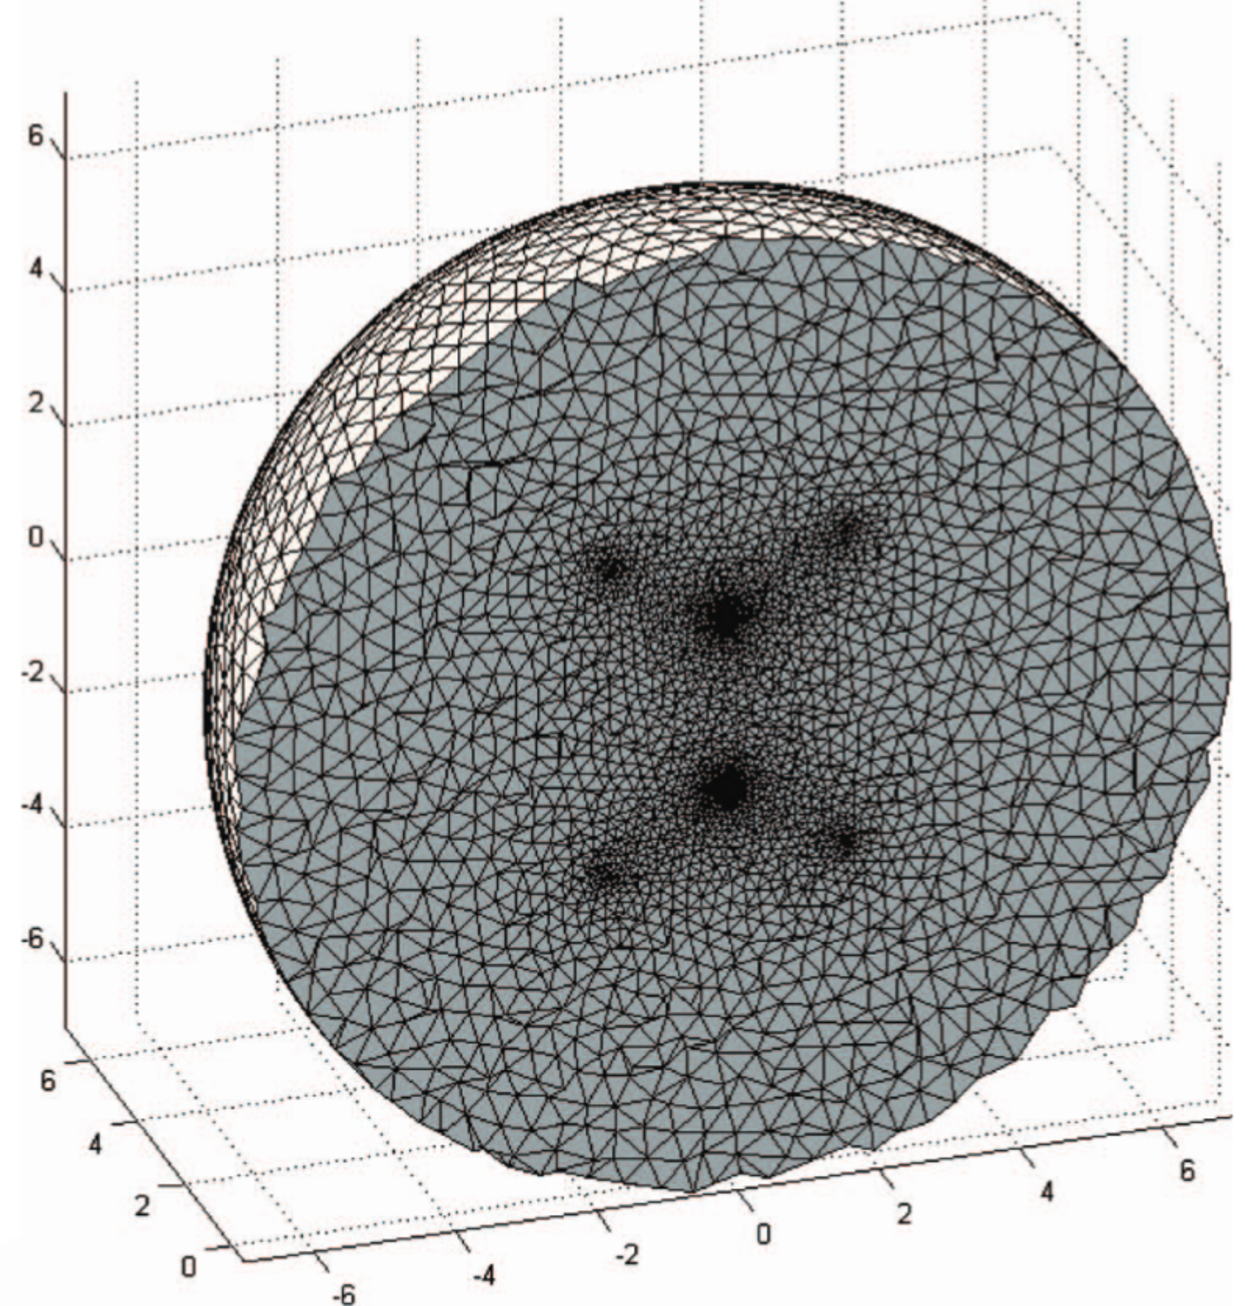
\includegraphics[width=\textwidth]{Figures/AdaptiveEthylene}
   \vspace{-44mm}\caption{$\qquad\quad\qquad\qquad$}
   \label{fig:AdapEthyl}
  \end{subfigure}
  \vspace{34mm}
  \caption{2D cuts through 3D meshes for molecular systems obtained with different schemes for local refinement:
    (a) hexahedral elements adapted for the benzene molecules \cite{fe_dft1}
    (b) hexahedral mesh for a diatomic \cite{fe_hf}
    (c) Polyhedral mesh for a benzene geometry \cite{fe_dft2}
    (d) Adaptive refined tetrahedral Mesh for ethylene. \cite{fe_hf}
    }
\end{figure}
The mesh obtained with this procedure for a benzene molecule \cite{fe_dft1} is shown in Figure \ref{fig:PolyBenz}.

When restricting oneself to tetrahedral elements, other design principles are possible: Since they are simplexes in three dimensions, they can be designed from general grids using, \textit{e.g.}, Voronoi \cite{voronoi} or Delaunay \cite{delaunay} tessellations %TODO:(the latter is described in section \ref{app:delaunay} in appendix) 
from a set of points with the required properties.
Son and Chu \cite{Son_Chu, Son_Chu0} constructed sets of points resembling molecular geometries by inserting $N$ spherical grids with different radii $r_i$ around the atoms and cutting off the overlapping regions.
The respective radii are chosen as
\begin{equation}
r_i=\frac{il}{N-i+\frac{lN}{r_\text{max}}} \qquad i=1,\hdots ,N 
\end{equation}
where $r_\text{max}$ is the radius of the largest sphere and $l$ is a parameter smoothly changing between a linear $l\rightarrow \infty$ and a $1/r$-mapping.
For the angular distribution of grid points they suggested the use of Lebedev-grids \cite{lebedev} and a Womersley design \cite{Womersley2001,Sloan}.
A more detailed discussion about the choices of grids is given in section \ref{sec:grid}.
%Choises for angular and radial grid distributions in this scheme are discussed in.% the chapters \ref{app:Sphere} and \ref{app:radius} respectively.

A more entangled method is used by Alizadegan \textit{et al.} \cite{fe_hf}. 
They start with an initial guess for the wave function and create a grid whose distances are inverse proportional to the second gradient of the electron density
\begin{equation}
d \propto \left[ \text{max}\left\{\left|\frac{\partial^2 \rho}{\partial x^2}\right| ,
                           \left|\frac{\partial^2 \rho}{\partial y^2}\right| ,
                           \left|\frac{\partial^2 \rho}{\partial z^2}\right| \right\} \right]^{-1}.
\end{equation}
which gives an estimate for the error due to linear approximation within each element.
After solving the eigenvalue equation on this grid, they recompute another mesh on the basis of the new function, iterating this procedure several times.
A cut through a mesh obtained by this procedure is shown in Figure \ref{fig:AdapEthyl}.

\section{Boundary Conditions}
\label{ch:BC}
Boundary conditions have not been addressed in this thesis so far for any of the methods but play an important role determining the properties of the solution.
In many cases, the boundary condition (BC) leads to uniqueness of the solution or at least it determines the branch to be searched as, \textit{e.g.} outgoing or incoming waves in case of the Helmholtz equation.
The simplest case is Dirichlet-boundary, requiring the wave function to vanish at the boundaries of a finite region.
In the FEM, this condition can be applied especially simple by setting the coefficients of the outermost shape functions to zero.
This truncation, however, strongly influences the wave function and discretises the spectrum since only an exact number of oscillations is allowed in the respective region.
To ensure a reasonably low error in energy, large domains are required.
Considering a particle with $1\,$eV kinetic energy, its wavelength is $~23\,$bohr.
To make the energy gap between two waves of the same angular momentum smaller than $0.1$eV, at least $10$ oscillations should fit in the radial direction, requiring a box-size of more than $230\,$bohr which is a unreasonably large sphere while kinetic energies in the $m$eV-range lead to even worse scenarios.
%Due to the large extend of the free particle, Dirichlet boundaries however are unphysical if they are not applied at distances that are several times larger than the wavelength.
%
%These considerations make clear that a more advanced boundary condition is needed which has only local influence on the wave function.
%In the following sub chapters, three boundaries that can be applied in FEMs are introduced and discussed.

Besides the numerical restriction to a finite box also mapping schemes can be used as \textit{e.g.} $x=\tan (\frac y2)$ that maps the range $[-\infty:\infty]$ to $[-\pi:\pi]$ \cite{PSbook}.
However, using such a mapping directly may lead to arbitrarily high oscillations and thus to arbitrarily sharp features in the mapped range. % and hence the representation of the FEF would still be poor.
Since the solution of unbounded differential equation occurs in many fields of physics and engineering, more sophisticated boundary conditions are available and the most important ones are presented in the following sections.

\subsection{Complex Absorbing Potential}
\label{ch:cap}
The complex absorbing potential (CAP) is a method often found in the literature when describing quantum-mechanical problems with infinite extent \cite{bauch1, bauch2,capWork}.
In this scheme, an artificial potential that is usually of quadratic form
\begin{equation} \label{eq:cap}
   W_\text{CAP}(\vec{r})=\begin{cases} -\text{i}\eta(\vec{r}-\vec{r}_0)^2 & ,\vec{r}>\vec{r}_0 \\
                                           0    &, \text{else} \end{cases}
\end{equation}
is added where the scaling $\eta$ is a free parameter and $\vec{r}_0$ is larger than the region where the solution is to be evaluated.
Such a potential damps the reflection of the wave function at the boarders and thus enhances the quality of states obtained on a finite region \cite{cap1, cap2} and can be shown to be equivalent to the complex scaling schemes that enjoy some popularity as well \cite{compScale,cap2,capWork}.
The imaginary potential (\ref{eq:cap}) leads to a non-hermitian term in the Hamiltonian and thus makes its eigenvalues complex whose real part corresponds to the energy of the respective state and the imaginary part is interpreted as its lifetime \cite{compScale}.

However, studies with different shapes of these potentials show that they influence the wave function not only close to the boarders and a proper design of the parameters is non-trivial \cite{CAPfreshlook}.
To minimise the error due to the CAP, the parameter $\eta$ can be chosen such that its dependency on the energy vanishes in first order, \textit{i,e.} $\eta\frac{dE}{d\eta}=0$ \cite{CAPccEOM,CAPfreshlook}.
If the parameter is chosen inappropriately, reflections or unstable resonances, making them strongly basis-set dependent, can occur \cite{CAPfreshlook}
%Moreover, due to non-hermiticity the usual scalar product is not suitable when calculating overlap integrals anymore.
Moreover, a dependence of the error on the frequency was observed \cite{babuska}.

%\subsection{Mode-matching Schemes}
\subsection{Non-Reflecting Boundary Conditions}
The term non-reflecting BC (or absorbing BC) describes a large class of BCs for problems on an infinite domain where it is subdivided into a finite computational domain and a residual infinite part that fulfils the requirement of not reflecting the solution back into the finite region of interest \cite{nrBCrev}.
Thus, also the previously described R-matrix approach (section \ref{ch:r-mat}) as well as the infinite elements described is section \ref{ch:InfEl} belong to this group of BCs.
There are also recently proposed approaches that are called perfectly matched layer schemes \cite{pmlBook,pml1, pml2}.

Absorbing BCs can in principle be applied to any kind of system but their applications are particularly prominent for the Helmholtz equation \cite{Engquist,HelmhPrec, nonreflectBC,nrBCrev}.
However, the problem of finding a reasonable non-reflecting BC is not yet solved for general case (\textit{i. e.} independent on symmetry and for other equations such as the Laplace equation) and is currently under investigation \cite{nonreflectBC,nrBCrev}.

As an example for a non-reflecting BC, the mode-matching scheme \cite{AstleyMM} is presented here which yields a particularly simple formalism.
In this scheme, the solutions of the Helmholtz problem in the finite inner region $\Gamma$ and infinite outer regions $\mathbb{R}^3\backslash \Gamma$ are considered as two separate functions, each described by the equations
\begin{equation}
   \label{eq:modeMatch}
   \nabla^2\Psi_1(\vec{r}) +V(\vec{r})\Psi_1(\vec{r})-E\Psi_1(\vec{r})=0 
\end{equation}
and
\begin{equation}
   \qquad \nabla^2\Psi_2(\vec{r}) -E\Psi_2(\vec{r})=0 
\end{equation}
whereby the outer function needs to satisfy the Sommerfeld condition \cite{sommerfeldCond} 
\begin{equation} \label{eq:Sommer}
\lim_{r\rightarrow\infty} r \left(\frac{\partial \Psi_2(r)}{\partial r} - \text{i}k \Psi_2  \right)\rightarrow 0
\end{equation}
along the radial direction $r=|\vec{r}|$ in three dimensions.
The quantities $\Psi_1(\vec{r})$ and $\Psi_2(\vec{r})$ are moreover coupled by 
\begin{equation}
\label{eq:modeCoup}
\Psi_1(\vec{r}_0)=\Psi_2(\vec{r}_0)  \qquad \text{and} \qquad 
\nabla \Psi_1(\vec{r}_0) \vec{n}=\nabla \Psi_2(\vec{r}_0) \vec{n}  \qquad \vec{r}_0 \in \partial \Gamma,
\end{equation}
where $\vec{n}$ is the normal vector on $\partial \Gamma$.
The \eqs{eq:modeCoup} ensure continuity of the solution and the gradient normal to the boundary \cite{AstleyMM}.
To ensure the Sommerfeld condition, one uses a respective basis in the outer region, \textit{e.g.} Spherical waves.
Using the mode-matching scheme with finite elements, the \eqs{eq:modeMatch} result in matrices similar to \eq{eq:SEmat} that are coupled by the conditions (\ref{eq:modeCoup}) that enter the weak formulation since the application of Greens' first identity in \eq{eq:SEweak} leads to an extra term.

\subsection{The Boundary Element Method}
The boundary element method (BEM) can be considered as a self-standing method for solving partial differential equations using the weak formulation \cite{bemDai,bemCostabel}.
The BEM is based on Greens' theorem, the Gau\ss-Ostrogradskii (divergence) theorem as well as Stokes theorem according to which all properties of a system can be projected onto its boundaries \cite{bemBook}.
In this method, thus, the partial-derivative equations are solved on the discretised boundaries only, leading typically to lower dimensional problems to be solved compared to volume-based methods such as the FEM.
However, the BEM scheme suffers strongly from the restriction of being applicable only to linear systems for which a fundamental solution is known.
In addition, the it leads to dense, unsymmetric matrix equations \cite{bemCostabel} which are numerically costly.
Still, this scheme enjoys up to now some popularity \cite{bem1,bem2,bem3}.
Its main advantages come into play when combined with the FEM \cite{bem-fem} to obtain an accurate solution in the inner region and the boundaries are treated with the BEM.
Considering an unbound domain as, \textit{e.g.}, the problem of the outgoing electron, the infinite domain $\Gamma$ can be divided into a finite region $\Gamma_i$ where the ionic ESP leads to a system-specific wave-function and the remaining domain $\Gamma_o$ in which the time-independent SE reduces to the Helmholtz-problem whose fundamental solutions are well-known.
Though the main conditions for the applicability of BEM are fulfilled for the problem of free electrons considered here \cite{bemCostabel, bettessBEM}.

\subsection{Infinite Elements}
\label{ch:InfEl}
The infinite element approach was developed in the 1980 for acoustical calculations and is specifically designed for the Helmholtz problem.
Moreover, it can be regarded as an extension of the BEM.
The general idea of the infinite elements is that the solution of the radial Helmholtz equation assuming spherical symmetry is known to be of the form
\begin{equation} \label{eq:infAnsatz}
 \Psi(r) = \left(\frac ar +\frac{b}{r^2} + \hdots \right) e^{ikr},
\end{equation}
where $k=|\vec{k}|$ is the absolute value of the momentum. 
Note that for the case of an outgoing photoelectron the prefactors $a$, $b$, \textit{etc.} correspond to different different angular momenta as can be seen by comparison with the Bessel function.
In the complete limit (for an infinite number of terms), any function fulfilling the Sommerfeld radiation condition \cite{sommerfeldCond} \eq{eq:Sommer} can be represented.

\begin{wrapfigure}{R}{0.5\textwidth}
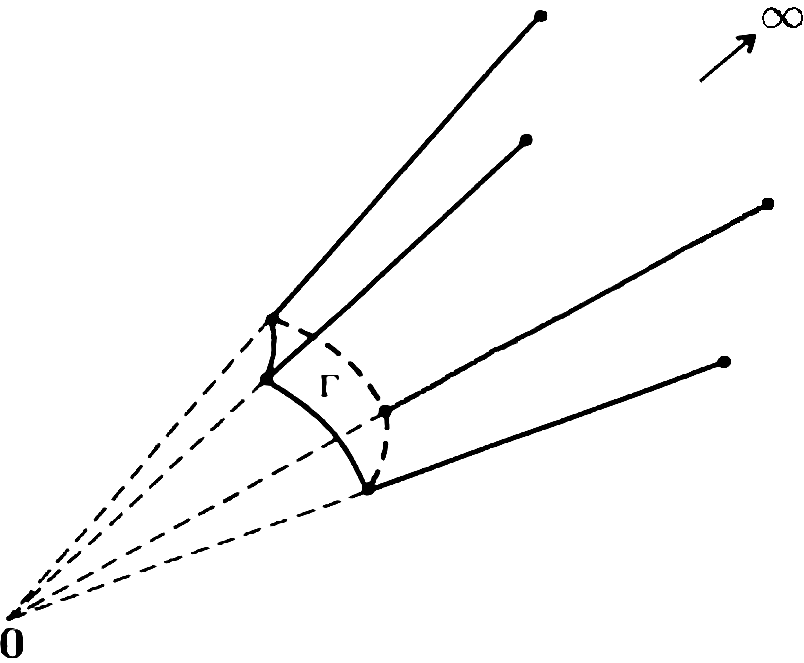
\includegraphics[width=0.5\textwidth]{Figures/BC/InfElem}
\caption{Schetch of an infinite element (solid lines).
Its front face $\Gamma$ coincides with the outer face of a finite element, the side faces are rays with a common centre. 
Figure adapted with modifications from \cite{dreyer}}
\label{fig:IElem}
\end{wrapfigure}
To use this asymptotic information, a single layer of elements is set onto the outer surface of the finite element region with shape functions of the form (\ref{eq:infAnsatz}).
To satisfy the continuity conditions, the front-face of these elements coincides with the outer face of the respective finite element, while their side faces have ray-like edges with a common centre in the middle of the finite element region as illustrated in Figure \ref{fig:IElem}.
In the graph, $\Gamma$ denotes the outer surface of the finite element region and the solid lines correspond to the edges of an infinite element.

Over the decades several formulations of infinite elements were developed making the ansatz for the solution of the form
\begin{equation} \label{eq:Infansatz}
 \Psi(\vec{r}) = \varphi(\vec{r}) e^{\text{i}k\mu(r)},
\end{equation}
where $\varphi(\vec{r})=f(r)\varphi_2(\vec{r}_\parallel)$ is a product of a transversal shape function $\varphi_2(\vec{r)}$ which depends only on coordinates $\vec{r}_\parallel$ parallel to the front face $\Gamma$ and a radial function depending only on the radial direction $r$.
Further, $\mu(r)=r-r_0$ where $r_0$ is the distance from the origin of infinite elements to the surface of the FEM region.
The function $f(r)$ is a multipole expansion \textit{i.e.} in terms of polynomials of $\frac{r_0}{r}$, where Jacobi-polynomials turned out to be the most stable basis \cite{dreyer_improved, infelNew}.
%The differences in the formulations are introduced by the test functions applied \cite{Astley}.
%An overwiev about different formulations is given in the references \cite{dreyer} and \cite{Astley}.
A number of different formulations have been introduced which differ in the form of the test functions.

As will be shown later, infinite elements result in a quadratic eigenvalue problem which is solved for the momentum $k$ and its square, respectively.
However, assuming that the difference between the eigenvalues of \eq{eq:SEinf} and the target energy of the outgoing electron is small, the quadratic eigenvalue problem can be approximated by the generalised eigenvalue problem (\ref{eq:SEmat}) by setting $k$ to the respective target momentum of the outgoing particle, reducing the computational cost.
%However, this approximation, which is applied here for simplicity, needs to be verified.

\subsubsection{Burnett Elements}
In the original Burnett formulation, the test functions are given in the form
\begin{equation} \label{eq:BUelem}
 \Phi(\vec{r}) = \varphi(\vec{r}) e^{-\text{i}k\mu(r)}.
\end{equation}
In the literature, usually the sign in the exponent is changed due to the use of another convention in the notation of the weak formulation \eq{eq:SEweak}.

Important is, however, that in the equation later on the test and ansatz functions enter both with same oscillatory factor, introducing oscillations with $e^{2ik(r-r_0)}$ in the Hamiltonian.
Thus, the resulting eigenproblem can be formulated as a non-linear problem by treating these oscillations as an unknown.
Alternatively, one sets $k$ to the target value, resulting in an energy-dependent Hamiltonian.
Even in the latter case, a quadratic eigenvalue problem remains which is non-hermitian.
Moreover it was found that this formulation can lead to numerical instabilities \cite{Astley} and to a wrong asymptotic behaviour.

To get rid of the oscillatory terms, in the unconjugated Burnett scheme the test functions can be chosen to coincide (in the notation used within this thesis) with the space of ansatz functions \eq{eq:Infansatz} and results in a symmetric quadratic eigenvalue problem.
However, the formulation of the Hamiltonian in this case is more complicated since the infinite integrals along the radial direction do not converge anymore \cite{Astley,gerdes}.
However, it can be shown that due to the symmetrisation of the kinetic energy term (see \eq{eq:SEweak}) additional surface integrals show up which lead to cancellation of the undefined terms \cite{gerdes}.
However, numerical tests comparing the conjugated and unconjugated formulations showed that the unconjugated elements \eq{eq:BUelem} have better convergence properties \cite{gerdes}.
%7This approach improves the numerical behaviour of the solution \cite{Astley} and yields an hermitian Hamiltonian.
%
%However, the volume integrals lead to infinite terms which are only cancelled by additional surface integrals arising \cite{gerdes}.
%Thus, the integrals are well-defined but numerically 
%Detailed numerical tests have shown that the conjugated Burnett elements are much more stable and accurate than the unconjugated scheme \cite{gerdes}.

\subsubsection{Asley-Leis Formulation}
Even though the conjugated Burnett elements do not perform that well, the conjugated infinite element formulation is appealing and can be expected to be numerically advantageous due to the cancellation of the infinite oscillations in the Hamiltonian.
Since the conjugated Burnett formulation seems to be not advantageous with the infinitely large contributions, in the Astley-Leis formulation the matrix elements are modified by an additional damping term in the infinite region.
Since the space of ansatz functions (\ref{eq:Infansatz}) corresponds to the multipole expansion of the outgoing waves, it should however not be modified.
To obtain a formulation with finite integrals with it, Astley suggested to chose test functions of the shape
\begin{equation} \label{eq:ALelem}
 \Phi(\vec{r}) = D(r)\varphi(\vec{r}) e^{\text{i}k\mu(r)},
\end{equation}
where in three dimensions $D(r)=\frac{1}{r^2}$ \cite{astley2}, leading to a non-symmetric Petrov-Galerkin scheme and a non-hermitian Hamiltonian.

Similar to the conjugated Burnett formulation, the resulting eigensystem does not have the energy as its eigenvalues but the generalised eigenvalue problem (\ref{eq:SEmat}) formulated in chapter \ref{ch:introFEM} changes to the quadratic eigenproblem
\begin{equation} \label{eq:SEinf}
\mat{A}\vec{c} +\text{i}k \mat{B}\vec{c}- k^2 \mat{C}\vec{c} =0 
\end{equation}
that is solved for the absolute value of the momentum $k=|\vec{k}|$.
The respective matrix elements are
\begin{align} \label{eq:InFEMmatrix}
\mat{A}_{i,j}& =\int \left(V(\vec{r}) D(r) \varphi_i(\vec{r}) \varphi_j(\vec{r}) 
                 +\frac 12 D'(r) \varphi_i(\vec{r})\varphi'_j(\vec{r})
                 +\frac 12 D(r) \varphi'_i(\vec{r})\varphi'_j(\vec{r}) \right) d\vec{r}\\
\mat{B}_{i,j}&=\frac 12 \int \mu'(r)\left(-D'(r) \varphi_i(\vec{r})\varphi_j(\vec{r})
                + D(r) \left(\varphi'_i(\vec{r})\varphi_j(\vec{r}) -\varphi_i(\vec{r})\varphi'_j(\vec{r})\right) \right) d\vec{r} \\
\mat{C}_{i,j}&= \frac 12 \int \left( \mu'(r) \mu'(r) + 1) D(r) \varphi_i(\vec{r}) \varphi_j(\vec{r})\right) d\vec{r}
\end{align}
where the prime is used as short-form of the spatial derivative and $r=|\vec{r}|$ is the distance to the origin of the infinite elements, moreover the relation $E=\frac 12 k^2$ is used \cite{dreyer}.

This formulation has been shown to be computationally robust for exterior acoustics \cite{dreyer_effectiveness,astley_stability}.
%The non-hermiticity of this Hamiltonian is, however, an important drawback of this formulation \cite{HamSelfAdj}.
The introduced imaginary part of the eigenvalue can be considered as a broadening due to the finite lifetime. %as well as an uncertainty of the energy.
%However, this is not very meaningful since the ansatz is done in practice in such a way that the wave function is not changed in an unphysical sense.
%To understand the respective results, here a symmetrised ansatz is suggested in the following.
However, this lifetime is not meaningfull since the damping function $D(r)$ is arbitrary.

\subsubsection{Symmetrised Formulation}
Besides those formulations mentioned above, further infinite element formulations are used \cite{dreyer}.
As an example, a variation of the Burnett-elements was applied to the harmonic oscillator \cite{bettessHarmonic} and (bound state) DFT calculations \cite{sobaMolecule} successfully.
Since bound states do not show oscillations but rather an exponential decay, the exponential function in the ansatz functions are modified to $-E_\text{IP}\mu(r)^2$ with the binding energy $E_\text{IP}$, respectively.
However, the application of infinite elements to FEFs is to the best of my knowledge a novelty of this work.

%Since the Astley-Leis elements suffer from their non-symmetric space of ansatz- and test-functions whereas the conjugate Burnett formulation has problems due to infinitely large matrix elements, here a symmetric but damped ansatz of the form
Astley-Leis and Burnett infinite elements have the main disadvantage of a non-hermitian Hamiltonian.
In this work, symmetric left and right basis functions are introduced, both being damped in the same manner:
\begin{align} \label{eq:ALsymm}
\Phi(\vec{r}) = \Psi(\vec{r}) = D(r)^p\varphi(\vec{r}) e^{ik\mu(r)}
\end{align}
Here, as before, $D(\vec{r})=\frac{1}{r^2}$ is taken but with the power $p>0$.
This provides more flexibility and ensures that the matrix elements are finite-valued and can be chosen to be, at least for small distances, similar to the analytic multipole expansion \eq{eq:Infansatz}.
The basis formulation (\ref{eq:ALsymm}) changes the mass and potential energy matrices in a trivial way whereas the kinetic energy matrix, which is in the original Astley-Leis formulation non-hermitian, becomes hermitian
\begin{multline} \label{eq:SymmKinE}
\int \left(\nabla \Phi^*_i(\vec{r})\right) \left(\nabla \Psi_j(\vec{r})\right) d\vec{r}=
%\int D^{2p}\Big(
%p^2 \frac{D'(r) D'(r)}{D^2(r)} +p \frac{D'(r)}{D(r)} \left(\varphi_i(\vec{r})\varphi'_j(\vec{r})+ \varphi'_i(\vec{r})\varphi_j(\vec{r}) \right)\\
%+ \left(  \varphi'_i(\vec{r})\varphi'_j(\vec{r}) + ik\mu'(r) \left(\varphi_i(\vec{r})\varphi'_j(\vec{r})- \varphi'_i(\vec{r})\varphi_j(\vec{r})  \right) -(ik\mu'(r))^2 \varphi_i(\vec{r})\varphi_i(\vec{r}) \right)
%\Big)d\vec{r}  
\int D^{2p}\Big(
\left|p \frac{D'(r)}{D(r)}- ik\mu'(r)\right|^2\varphi_i(\vec{r})\varphi_j(\vec{r}) 
+p \frac{D'(r)}{D(r)} \left(\varphi_i(\vec{r})\varphi_j(\vec{r})\right)'\\
+ ik\mu'(r) \left(\varphi_i(\vec{r})\varphi'_j(\vec{r})\right)+ \varphi_i'(\vec{r})\varphi_j'(\vec{r})
\Big)d\vec{r}  
\end{multline}
This is the main working equation in this work.
Symmetric left and right bases ensure hermiticity of the problem and thus real-valued energies of the outgoing electron.
In principle, any arbitrary small $p>0$ is enough to make the integrals over the infinite elements finite.
Chosing it quite small one mitigates the suppression of fewer angular momenta as discussed in section \ref{sec:iBCbench}.

\section{Solving Large Eigenvalue Problems}
\label{ch:ghep}
In finite element applications such as those being proposed in this work, matrix equations with hundreds up to hundred thousands of dimensions need to be solved.
This requires elaborate strategies, using the sparsity of these matrices.

The focus here is on solving the generalised eigenvalue problem (\ref{eq:SEmat}) and the quadratic problem (\ref{eq:SEinf}) respectively.
However, efficient strategies are only known for regular eigenvalue problems of the form 
\begin{equation} \label{eq:eigenprob}
\mat{A}\vec{x}=\lambda\vec{x}.
\end{equation}
Hence, the more general forms will be rewritten to become (\ref{eq:eigenprob}) as discussed in section \ref{ch:GenEV}.
Moreover, since the state of interest is an unbound state, one expects a high density of states. 
This, however, is a well-known problem in numerical mathematics since almost degenerate eigenvalues and especially their respective eigenvectors are very sensitive to small perturbations iin matrix $\mat{A}$.
Section \ref{ch:regular} addresses these problems and a way for numerical stabilisation is sketched.
Finally in section \ref{ch:ghep} few methods are presented showing how a small number of approximate eigenpairs can be obtained in a numerically efficient way from the usual eigenproblem (\ref{eq:eigenprob}).

For the computation of eigenpairs, many classes of solvers have been developed with various numerical properties.
Besides direct solvers such as the Gau\ss-elimination, iterative solvers are to be mentioned that are especially well-suited for large but sparse equation systems.
Besides the famous Jacobi- and Gau\ss-Seidel algorithms which converge only in certain cases, also the Davidson method \cite{davidson,davidson2} and several Krylov subspace methods \cite{krylov1,krylov2} are commonly used.
For finite element problems, the Krylov subspace solvers turned out to be a very efficient class \cite{slepcManual,FEMsolvers}.

As discussed in the sections \ref{ch:GenEV} and \ref{ch:regular}, the solution of a generalised eigenvalue problem involves undesireable matrix operations which destroy their sparse structure.
As a popular choice for such classes of problems, the Krylov subspace is used.
A $q$-dimensional Krylov subspace is generated by a vector $\vec{x}$ and a matrix $\mat{A}$ and has the form
\begin{equation}
   \mathcal{K}_q(\mat{A},\vec{x})=\text{span}\left\{ \vec{x},\mat{A}\vec{x},\mat{A}^2\vec{x},\hdots,\mat{A}^{q-1}\vec{b} \right\}.
\end{equation}
If $\mat{A}$ is sparse, the evaluation of these expressions is only of order $\mathcal{O}(d)$, where $d$ is the dimensionality of $\vec{x}$.
The vectors obtained with large powers of $\mat{A}$, however, become more and more linearly dependent.
To prevent this, the vectors usually are orthonormalised inbetween.
The orthogonalisation method being used distinguishes different Krylov subspace methods such as the Arnoldi \cite{str-4} or Lanczos schemes \cite{str-5}.
In this work, the Krylov-Schur algorithm is used \cite{str-7,KrSch}.
An important issue in this scheme is a good choice for $\vec{x}$ which crucially determines the speed of convergence.
If a reasonable starting-vector cannot be guessed, the space $\mathcal{K}_q$ needs to be extended by increasing $q$ iteratively.
To keep the dimensionality low, in this algorithm the subspace iteration is restarted after $q$ reached a certain value, starting with a better guess $\vec{x}$.
%The efficient restart is another critical issue in this scheme.
%In the Krylov-Schur algorithm \cite{KrSch} used here, the restart is conducted implicitly as described in more detail in ref. \cite{str-7}.

%\subsubsection{Inverse iteration and Power methods}
%not suitable for the initial problem, but maybe for the transformed one?
%How well do they work if only an approximate eigenvalue is known?
%
%\subsubsection{Arnoldi, ... Methods}
%
%more description and some explanations on convergence, compared to other methods etc.: http://onlinelibrary.wiley.com/doi/10.1002/gamm.201490008/pdf
% http://www.ams.org/journals/mcom/1981-37-155/S0025-5718-1981-0616364-6/
% GRMES description: http://epubs.siam.org/doi/abs/10.1137/0907058
%
% alternative: Jacobi-Davidson: http://epubs.siam.org/doi/abs/10.1137/S0036144599363084
% general overview: http://www.sciencedirect.com/science/article/pii/S0377042700004131
%
%How is this inversion done numerically?
%
%\subsection{Quadratic Eigenproblem}
%\label{ch:quadEV}
%--> Probably this chapter is not of interest here since I don't use the respective formulation!?

\subsection{Generalised Eigenproblem}
\label{ch:GenEV}
The most straightforward way to reformulate the generalised eigenvalue problem
\begin{equation} \label{eq:Gep}
\mat{A}\vec{x}=\lambda\mat{B}\vec{x},
\end{equation}
where left left and right bases are not orthonormal with the overlap matrix $\mat{B}$ is the invert the matrix $\mat{B}$, obtaining the regular Eigenproblem $\mat{B}^{-1}\mat{A}\vec{x}=\lambda\vec{x}$.
This inversion corresponds to the orthogonalisation of the left basis with respect to the right one but is possible only as long as $\mat{B}$ is invertible and not too large since inversion is a demanding operation.
Moreover, the initial matrices are sparse but $\mat{B}^{-1}\mat{A}$ looses its sparseness \cite{slepcManual}.

To prevent the appearance of dense matrices, mathematical computer libraries often do not operate with the matrices themselves but rather with a set of vectors on which these matrices act \cite{slepcManual}.
The most popular scheme of this kind is the Rayleigh-Ritz projection where the initial problem is reduced to a smaller subspace $\mathcal{V}_j=\text{span} \{\vec{v}_1,\hdots,\vec{v}_j\}$ of dimensionality $j$, spanned by appropriate vectors $\vec{v}_i$.

Projecting the \eq{eq:Gep} onto $\mathcal{V}_j$ yields the new system $\mat{\Sigma}_j \vec{s}=\theta\mat{\Theta}_j\vec{s}$ where $\mat{\Sigma}_j=\mat{V}_j^T\mat{A}\mat{V}_j$ and $\mat{\Theta}_j=\mat{V}_j^T\mat{B}\mat{V}_j$.
The matrix $\mat{V}_j$ is unitary with the rows $(\mat{V}_j)_i=\vec{v}_i$.
After solving this dense but small problem, the original eigenvectors can be approximated as $\vec{x}_j=\mat{V}_j\vec{s}_j$ and $\lambda=\theta_j$.
The obtained eigenpair is a good approximation to the actual one as long as the subspace $\mathcal{V}_j$ contains the respective solution or contains a vector which is at least close to it.

\subsection{Regularisation of Eigenproblems}
\label{ch:regular}
Independent of the efficiency and robustness of the eigensolver in use, seeking solutions of the SE for free particles in continuum means that eigenenergies are very close to each other or even highly degenerate.
Such dense-lying eigenvalues lead to numerical difficulties and especially the eigenvectors are known to be unreliable in this case.
In practice, this means that the iterative schemes do not converge anymore, requiring a reformulation of the mathematical problem.

One way to circumvent these instabilities is to reformulate it as a minimisation problem \cite{H2pDeCleva}.
Therefore \eq{eq:SEmat2} is rewritten as $\left(\frac 12 \mat{A}+\mat{V} - E \mat{M}\right)\vec{c}_i = 0$ and is set prior to minimisation where the parameter $E$ is the target energy.
Since this does not give an ambiguous solution, one minimises the residual of the desired solution
\begin{equation}
\text{min}_{||\vec{x}||=1}\left\{\left|\left|\left(\frac 12 \mat{A}+\mat{V}-E\mat{M}\right)\vec{x} \right|\right| \right\}.
\end{equation}
Using the $L_2$-norm, it is equivalent to finding the smallest eigenvalue of
\begin{equation} \label{eq:SEmin}
\left(\frac 12 \mat{A}+\mat{V}-E\mat{M}\right)^\dagger
\left(\frac 12 \mat{A}+\mat{V}-E\mat{M}\right) \vec{x}_i = \theta \vec{x}_i,
\end{equation}
where $\theta$ is a measure for the error in energy.
%To avoid the costly multiplication of two matrices, one can use  Hermiticity of the matrices and take compute the
%square root as
%\begin{equation} \label{eq:SEmin}
%\left(\frac 12 \mat{A}+\mat{V}-E\mat{M}\right)\vec{c}_i = \lambda \vec{c}_i
%\end{equation}
%which is a usual eigenvalue problem \cite{H2pDeCleva} and $\lambda$ with smallest absolute value is searched.
%
%Nonetheless, the latter formulation is only an approximation as the comparison of (\ref{eq:Gep}) and (\ref{eq:SEmin}) shows, the latter approximates the mass matrix$\mat{M}$ as unity $\mat{1}$.
%Furthermore, \eq (\ref{eq:SEmin}) still is expected to have a very dense spectrum and $\lambda$ is an interior eigenvalue so the initial problem is not expected to be solved in this approach.
Whereas \eq{eq:SEmin} is only an approximation to the original problem, it has the advantage that it is a quadratic expression in the matrices which lead to a more stable behaviour \cite{H2pDeCleva}.

Similar schemes which are reformulations of the original problem are often referred to as spectral transformations \cite{slepcManual}.
One example is the harmonic extraction, where the eigenvalues of original expression (\ref{eq:Gep}) are first shifted such that the target value is $0$, leading to the equation 
\begin{equation} \label{eq:Shift}
\left(\mat{A}-\tilde{\lambda}\mat{M}\right)\vec{x}=(\lambda-\tilde{\lambda})\mat{M}\vec{x}
\end{equation}
where $\tilde{\lambda}$ is the target value of the original problem.
Then, the equation is multiplied by $\mat{A}-\tilde{\lambda}\mat{M}$, resulting in the equation 
\begin{equation}
\left(\mat{A}-\tilde{\lambda}\mat{M}\right)\left(\mat{A}-\tilde{\lambda}\mat{M}\right)\vec{x}=(\lambda-\tilde{\lambda})\left(\mat{A}-\tilde{\lambda}\mat{M}\right)\mat{M}\vec{x}
\end{equation}
which is observed to lead to faster convergence for Krylov-subspace methods \cite{slepcManual,harmExt}.

Other spectral transformations are the spectral folding \cite{slepcManual} where the left and right sides of \eq{eq:Shift} are squared respectively which often leads to higher stability but the squaring of eigenvalues leads to ambiguities with respect to the eigenvalues $\lambda$ of the original problem.
%Instead of the reformulation, here a regularisation of the problem used, applying the spectral transformation shift and invert.
%Starting thit the problem: $\mat{A}\vec{x}=\lambda\mat{B}\vec{x}$ where the eigenvalues closest to the target energy $\varepsilon$ are of interest, the spectrum can be shifted to a target energy of $0$ by
%\begin{equation}
%\left(\mat{A}-\varepsilon\mat{B}\right)\vec{x}=(\lambda-\varepsilon)\mat{B}\vec{x}
%\end{equation}
The scheme that turned out to be most beneficial for the matrices used in this work is the shift-and-invert scheme where the inverted problem of \eq{eq:Shift}, \textit{i.e.}
\begin{equation}\label{eq:stSI}
\left(\mat{A}-\tilde{\lambda}\mat{M}\right)^{-1}\mat{M}\vec{x}=\frac{1}{\lambda-\tilde{\lambda}}\vec{x},
\end{equation}
is solved. 
The formulation (\ref{eq:stSI}) has the advantage that the transformed eigenvalues $\frac{1}{\lambda-\tilde{\lambda}}$ are well-separated and on the extrema of the new spectrum, \textit{i.e.} they approach $+\infty$ and $-\infty$ if $\tilde{\lambda}$ is inbetween two eigenvalues.
Since the Krylov-scheme is especially efficient when the largest or smallest eigenvalues need to be found, this leads to faster convergence and to a more stable procedure due to the separation of eigenvalues \cite{str-7}.
A more generalised transformation is the Cayley-transform which has two parameters $\tilde{\lambda}$ and $\tilde{\tilde{\lambda}}$ and yields the usual eigenvalue problem
\begin{equation}
\left(\mat{A}-\tilde{\lambda}\mat{M}\right)^{-1}\left(\mat{A}+\tilde{\tilde{\lambda}}\mat{M}\right)\vec{x}=\frac{\lambda+\tilde{\tilde{\lambda}}}{\lambda-\tilde{\lambda}}\vec{x}.
\end{equation}

Finally, a regularisation of eigenvalue problems can be performed using matrix preconditioners.
Many different types of preconditioners are developed \cite{Helmke2010} but most of them are efficient only for a small class of problems.
For instance, algorithms especially well-suited for matrices originating from FEM-problems have been suggested \cite{PrecFem, PrecFem2}, which can be even adapted to a FEM structure \cite{MultPrec,MultPrec2} or to a particular physical problem \cite{HelmhPrec}. 
Often their performance notably depends on the eigenproblem solver \cite{PrecKr}.
This fact makes their efficient use more intricate and can easily lead to higher costs than the actual benefit.
In this thesis, the shift-and-invert scheme (\ref{eq:stSI}) is used for all the calculations obtained and discussed in chapter \ref{ch:res}.

